The main contribution of this thesis is represented by the design of a toolchain for Graph Neural Network acceleration on FPGA leveraging High-Level Synthesis.

This chapter explains in detail how the toolchain has been designed and how it can be used to build GNN accelerators to enhance inference performance.

The core component of the toolchain is the synthesizer, enclosing SODA-OPT~\cite{9786533} and PandA-Bambu~\cite{9586110}, upon which the research team responsible for supervising this thesis has dedicated significant efforts over the past years.
The primary objective of this thesis is to enhance SODA-OPT and Bambu to bridge GNN models written in high-level frameworks, such as PyTorch, to FPGA architectures.

Figure~\ref{fig:toolchain} illustrates the entire design flow, with the steps involved in the GNN acceleration process.
In particular, firstly, the GNN model is implemented in PyTorch, one of the most popular and powerful frameworks for Neural Network implementations.
Subsequently, the model is passed as input to Torch-MLIR, a crucial middle step that enables the generation of the MLIR representation.
This intermediate representation serves as input for the synthesizer, where, once the frontend optimization is complete, the refined version proceeds to the backend, where the actual GNN accelerator is effectively produced, ready to enhance inference performance on FPGA architectures.

The following Sections provide a comprehensive and in-depth exploration of each step within the proposed design flow.
This detailed breakdown highlights the various possibilities inherent in the toolchain and outlines the recommended procedures necessary to achieve the optimal outcome for GNN acceleration.
The thesis aims to equip researchers and practitioners in Graph Neural Networks with the necessary insights and understanding to harness the full potential of this toolchain and unleash the power of FPGA acceleration.

In conclusion, this thesis represents a significant advancement in Graph Neural Network acceleration.
By designing a refined toolchain and bridging the gap between high-level frameworks and FPGA architectures, this research contributes to the broader field of artificial intelligence.
It reinforces the potential of FPGA-based accelerators in revolutionizing the inference performance of GNN models.
The implications of this work offer a solid foundation for further exploration and advancements in the field of hardware acceleration for deep learning applications.

\begin{figure}[t]
    \centering
    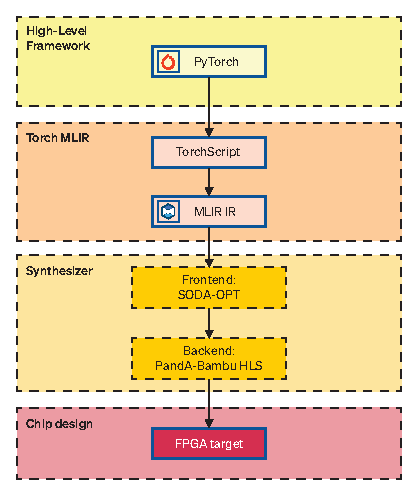
\includegraphics[height=0.6\textwidth]{Images/toolchain}
    \caption{FPGA Toolchain for Graph Neural Network Acceleration}
    \label{fig:toolchain}
\end{figure}

\section{PyTorch}
\label{sec:toolchain-pytorch}%

PyTorch~\cite{DBLP:journals/corr/abs-1912-01703} is an open-source deep learning framework widely used for building and training artificial neural networks for various machine learning tasks.

The first step of the toolchain is to design and implement the Graph Neural Network model in PyTorch.
Doing so involves defining the GNN model architecture and writing the necessary forward pass to compute node and graph-level representations.
Once having defined the model, the next step is training the GNN using standard PyTorch techniques, such as defining a loss function, setting up an optimizer, and performing backpropagation to optimize the model parameters.

\subsection{GNN models}
\label{subsec:gnn_models}%

Two main models have been used for this thesis: the Graph Isomorphism Network from OGB~\cite{NEURIPS2020_fb60d411, ogb_gnn_models}, written using PyTorch Geometric~\cite{DBLP:journals/corr/abs-1903-02428}, and the Graph Convolutional Network~\cite{DBLP:journals/corr/KipfW16, pygcn}, written using PyTorch~\cite{DBLP:journals/corr/abs-1912-01703}.

Most research and experiments have been conducted using the GCN model.
The GCN class is characterized by two Graph Convolutional layers, and the forward function of each layer is mainly characterized by two matrix multiplications.


\subsection{Datasets}
\label{subsec:gnn_datasets}%

OGB provides different datasets that can be used with their models.
The one used for this thesis is called \textit{ogbg-molhiv}, a molecular property prediction dataset.
In each graph representing a molecule, nodes correspond to atoms, and edges represent chemical bonds.
The input node features consist of nine dimensions, encompassing information like atomic number, formal charge, and whether the atom is part of a ring.
The binary classification task consists in achieving precise predictions of target molecular properties, for example, determining whether a molecule inhibits HIV replication or not.

The dataset used for the GCN model is the \textit{Cora} one.
This dataset contains 2708 scientific publications, categorized into one of the seven classes considered.
The citation network contains 5429 links.
Each publication in the dataset is represented by a binary-valued word vector, indicating the absence or presence of the corresponding word from a dictionary of 1433 unique words.
The task is a multiclass classification, in which, given a paper, the objective is to classify it into one of the seven classes correctly.

\section{Torch-MLIR}
\label{sec:toolchain-torch_mlir}%

Torch-MLIR~\cite{torch_mlir} offers compiler support for transitioning from the PyTorch ecosystem to the MLIR ecosystem.

The steps Torch-MLIR follows to go from PyTorch to MLIR are shown in Figure~\ref{fig:torch-mlir}.
In particular, the flow followed in this thesis has been highlighted with blue arrows.
There are two starting points of the flow: TorchScript and LazyTensorCode.
The one used for this research, which is also the most tested one, is TorchScript.
TorchScript~\cite{torchscript} offers a way to generate serializable and optimizable models directly from PyTorch code.

The TorchScript representation is then converted to MLIR using the built-in conversion of Torch-MLIR. The result MLIR can use different dialects, but the one used for this thesis is the Linalg dialect, which serves as input for the next phase of the toolchain.

\begin{figure}[t]
    \centering
    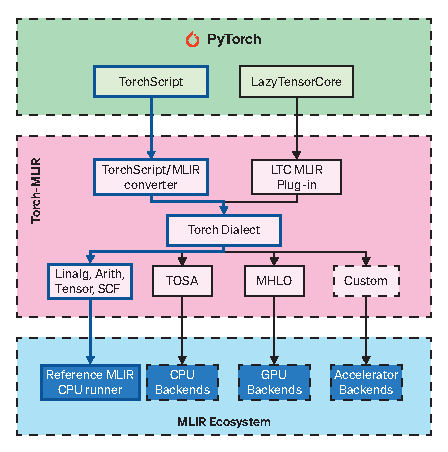
\includegraphics[height=0.5\textwidth]{Images/torch-mlir}
    \caption{Torch-MLIR flow}
    \label{fig:torch-mlir}
\end{figure}

\subsection{From PyTorch to TorchScript}
\label{subsec:pytorch-to-torchscript}%

Since Torch-MLIR implicitly uses the TorchScript representation to go from PyTorch to MLIR, the first part of the research consisted of a deep analysis of the Graph Neural Network models to make them compatible with TorchScript.

This task required more effort for the GIN model due to its use of PyTorch Geometric than the GCN model, which only uses pure PyTorch.
In particular, the required adaptations, that have been used for both models, have been made general aiming to make them versatile for various applications.
They are documented below, with a small example for each of them:

\begin{itemize}
    \item[-] The GNN layer class, if created as a subclass of the Message Passing class, must be marked as Jittable whenever it is used.
\begin{lstlisting}[language=Python,label={lst:jittable}]
self.convs.append(GINConv(emb_dim).jittable())
\end{lstlisting}
    \item[-] The propagate function, if used, need its parameters to be explicitly annotated using one of the two available options: through the definition of a dictionary or through a comment.
\begin{lstlisting}[language=Python,label={lst:propagate-annotation}]
propagate_type = {'x': Tensor, 'edge_attr': Tensor}
\end{lstlisting}
    \item[-] It can happen that TorchScript is not able to recognize the correct type of variables.
    In this case, it is necessary to use an assertion to explicitly declare that the variable is an instance of the correct type.
\begin{lstlisting}[language=Python,label={lst:isinstance-assertion}]
assert isinstance(edge_embedding, Tensor)
\end{lstlisting}
    \item[-] A common approach to speed up the training and inference steps is to use batched data.
    Unfortunately, TorchScript does not support forward functions that take as input a batch.
    For this reason, the forward function must receive Tensors as input, thus the batch must be split into its component.
\begin{lstlisting}[language=Python,label={lst:splitted-forward}]
def forward(self, x, edge_index, edge_attr):
\end{lstlisting}
    \item[-] The parameters of the forward function must be explicitly annotated with their type.
    If not declared, it is assumed to be of type Tensor.
\begin{lstlisting}[language=Python,label={lst:forward-annotation}]
def forward(self, x: Tensor, edge_index: Tensor,
            edge_attr: Tensor) -> Tensor:
\end{lstlisting}
    \item[-] TorchScript always expects an integer literal for the index, this is because indexing is only supported with integer literals.
    For this reason, cycles that do not use integer literals must be changed into enumeration.
\begin{lstlisting}[language=Python,label={lst:enumeration}]
for idx, layer in enumerate(self.convs):
\end{lstlisting}
\end{itemize}

\subsection{Torch-MLIR Compilation}
\label{subsec:torch-mlir-compilation}%

Once having designed, implemented, made compatible with TorchScript, and trained the GNN model in PyTorch, it is possible to use the \lstinline{torch_mlir.compile} API to obtain the MLIR representation of the model.
In particular, this API takes three parameters as input: the GNN model, an input example of the model and the desired output type.
The Graph Neural Network model must have been already trained, being ready for inference.
The second parameter, the input example of the model, is an arbitrary input similar to the one that would be given for inference purposes.
It is required because, by default, the implicit Jit function called by Torch-MLIR to script the model and obtain a script module, involves compiling the forward method and recursively compiling any methods, submodules, and functions called within the forward method. This results in a JIT IR which is converted to the torch dialect which is almost in a 1:1 correspondence.
The torch dialect is then lowered into one of the three available output dialects: linalg, tosa, mhlo.
The purpose of the last parameter is to choose which of these three dialects has to be used for the output MLIR.

An additional parameter that can be used is related to the tracing.
There are two ways in which it is possible to obtain a TorchScript representation: \lstinline{torch.jit.script} and \lstinline{torch.jit.tracing}.
The compile API of Torch-MLIR uses the first one by default.
Instead, if the option use tracing is set to True, JIT tracing is used.
The behavior of the two functions is slightly different.
Tracing only captures functions and modules that lack data dependencies and untracked external dependencies.
It records operations performed when the specified function is executed on the given tensors.
As a result, the resulting ScriptModule consistently executes the same traced graph for any input.
In conclusion, tracing can be a valid option in some cases, such as when there is no need to record any control-flow like if-statements or loops, but the scripting is preferred, and it is guaranteed to work in a more wide set of cases.
A call example of the compile Python API of Torch-MLIR is reported below.
\begin{lstlisting}[language=Python,label={lst:torch_mlir-compile}]
module = torch_mlir.compile(gnn_model, (x, features, adj),
                            output_type="linalg-on-tensors")
\end{lstlisting}

Once having obtained the compiled module, the expected behavior is to use one of the backends provided by torch-MLIR to make the inference.
This is not the flow followed in this thesis, because, as represented in the accelerator design flow, in Figure~\ref{fig:toolchain}, it is needed to export the Linalg representation for the next phase.
This can be done by simply saving the model to an MLIR file, as shown below.
\begin{lstlisting}[language=Python,label={lst:torch_mlir-export}]
with open("gnn_model.mlir", "w", encoding="utf-8") as outf:
    outf.write(str(module))
\end{lstlisting}

Only the GCN model implemented in PyTorch reached this phase of the toolchain.
During the research, much effort has been spent in trying to add support for the PyTorch Geometric framework to the toolchain.
Even if some innovation has been brought in this regard, there are still open points to work on.
For this reason, at the actual state, the proposed design flow only supports PyTorch as a high-level framework
It must be noted that no documentation existed and no previous works have ever used Torch-MLIR with GNN models.
All the examples and the work done by the Torch-MLIR community are related to Deep Neural Network models.

This thesis could represent the first work that explored the use of Torch-MLIR with GNN models.
Unfortunately, even if some innovation has been brought, such as the implementation of support of the constant of Tuple type, some more work is still required.
In particular, Torch-MLIR does not support the \lstinline{aten.scatter_add} operation, which, at the actual state, cannot be lowered to MLIR\@.
This operation is extensively used by PyTorch Geometric, leading to the incompatibility of the two elements.
The next step to add support for PyTorch Geometric to the proposed toolchain would be the implementation to Torch-MLIR of the lowering of the scatter add operation.

Another point discovered during this thesis is the fact that Torch-MLIR does not support the sparse tensor type. 
Each sparse tensor implemented in PyTorch, with the relative sparse operations, is lowered to MLIR to a dense tensor, losing all its representation's advantages.
A promising option to avoid this is Taco~\cite{taco} with its PyTaco APIs for Python.
The MLIR team started creating what is called MLIR-PyTACO~\cite{mlir-pytaco}, an end-to-end use case for the sparse tensor compiler, which can be used to lower sparse Tensor to MLIR\@.
It is important to clarify that, as introduced in~\cite{Bik_2022}, sparse tensors are supported by MLIR, with a dedicated sparse tensor dialect that uses intuitive annotations for different sparse tensor representations, such as CSR and COO.
What is not supported yet is the lowering through Torch-MLIR\@.
However, even if MLIR-PyTACO is still premature and in testing phase, interesting features could be brought by its advancement.

Even losing the sparse tensor representation, using the proper optimizations provided by the toolchain in combination with the higher computational performance of FPGAs, still make it possible to accelerate the GNN operations, as will be stated in the next Chapter.

\section{Synthesizer}
\label{sec:toolchain-synthesizer}%

The synthesizer represents the final step of the toolchain, which optimizes and synthesizes the MLIR representation, targeting FPGA\@.
This step includes SODA-OPT and PandA-Bambu, both introduced in Section~\ref{sec:soda}.
The following Subsections provide insight into what is happening internally to these two components.

\begin{figure}[t]
    \centering
    \subfloat[Compiler frontend\label{fig:soda-opt_flow}]{
        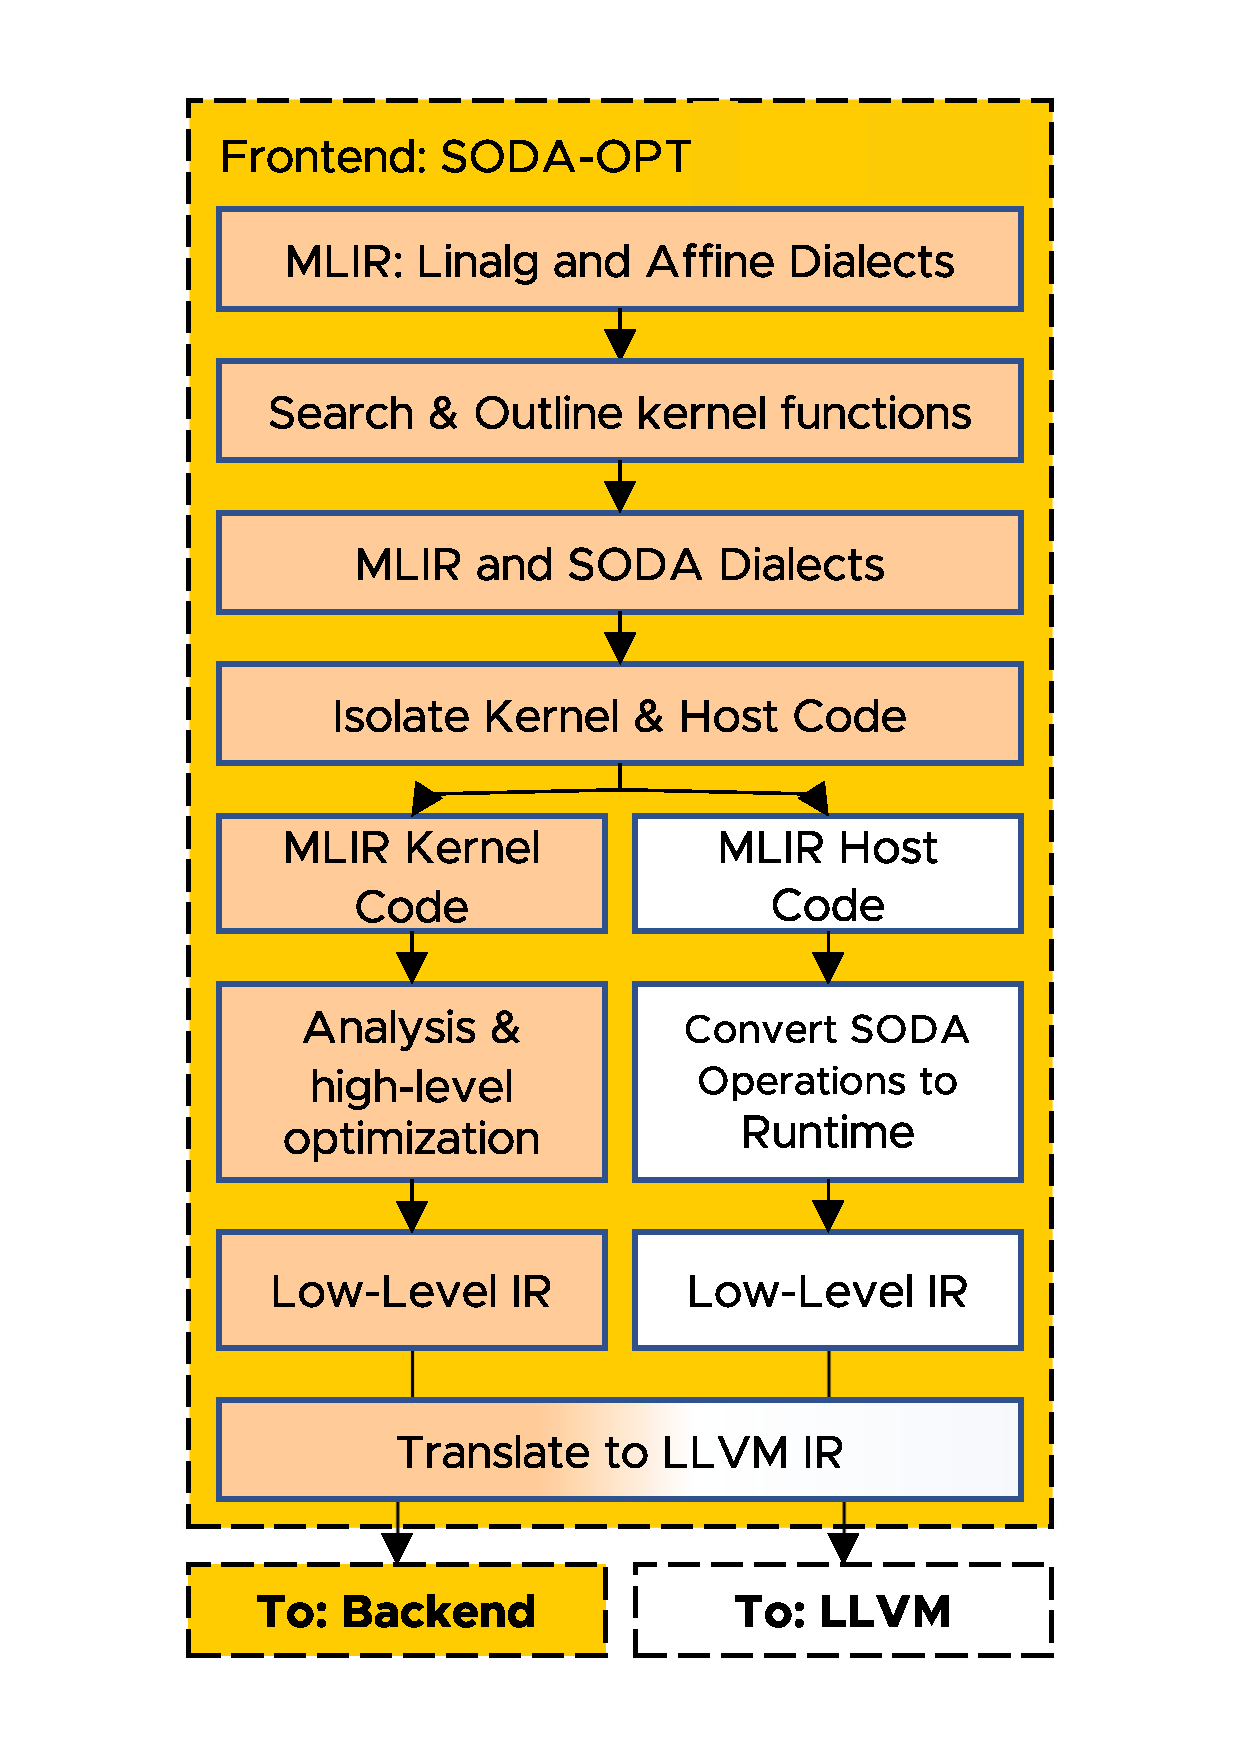
\includegraphics[height=0.6\textwidth]{Images/soda_opt_flow}
    }
    %\quad
    \hspace{0.03\textwidth}
    \subfloat[High-level synthesis backend\label{fig:bambu_flow}]{
        \captionsetup{width=.4\textwidth}
        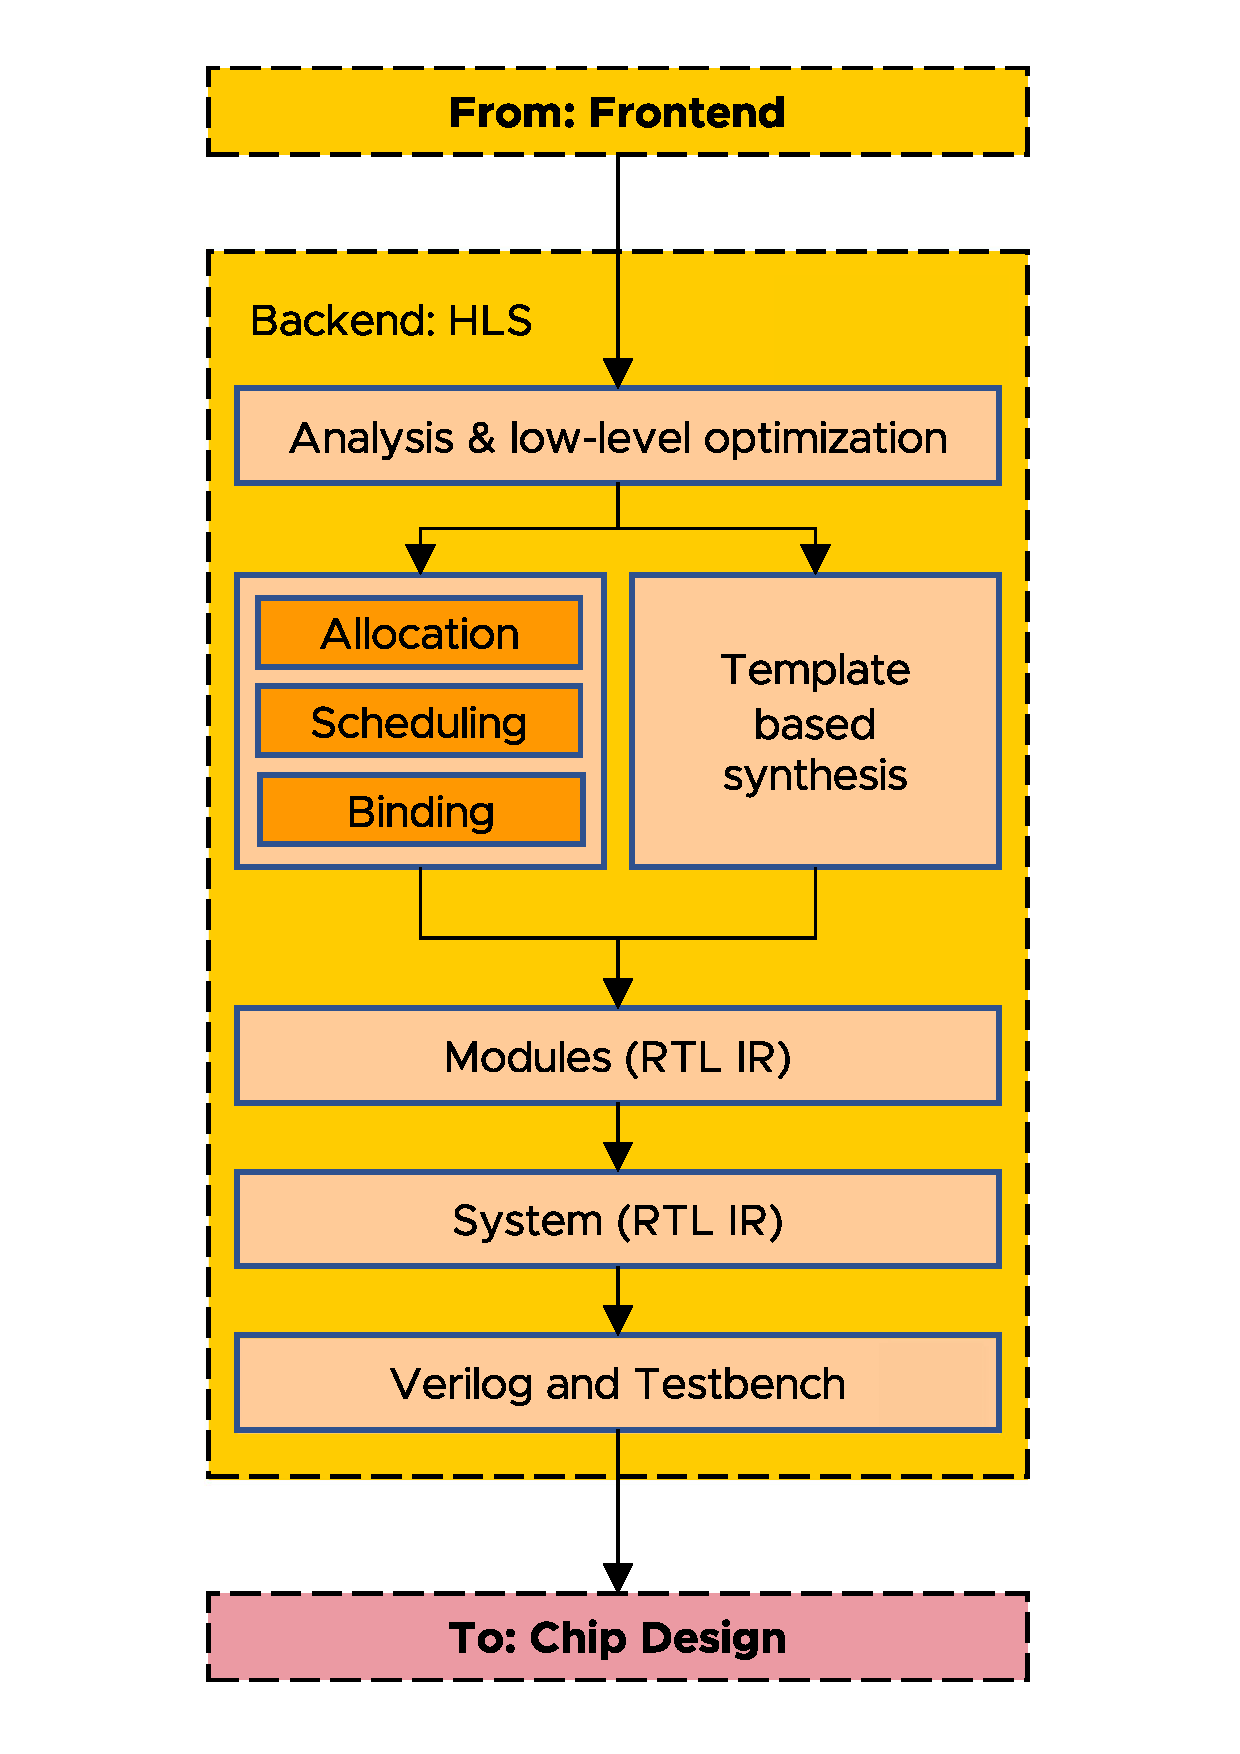
\includegraphics[height=0.6\textwidth]{Images/bambu_flow}
    }
    \caption{Synthesizer: SODA-OPT and PandA-Bambu overview~\cite{9786533}}
    \label{fig:synthesizer_flow}
\end{figure}

\subsection{SODA-OPT}
\label{subsec:toolchain-soda_opt}%

SODA-OPT, as shown in Figure~\ref{fig:soda-opt_flow}, receives as input the MLIR representation of the model.
This step is primarily responsible for applying optimizations that can be exploited in the next step.
In particular, a subset of MLIR passes can be used to do so.
The output of SODA-OPT is an LLVM representation that serves as input to PandA-Bambu HLS\@.

Despite the remarkable capabilities of SODA-OPT, it should be noted that it does not support the entire set of dialects utilized within the MLIR ecosystem, such as the ml\_program or the Tensor dialect.
Consequently, an additional step is required wherein the representation obtained from Torch-MLIR is lowered to remove unsupported dialects.
In particular, once having successfully exported the MLIR representation using the \lstinline{torch_mlir.compile} API, a set of mlir-opt passes have been used to remove the unsupported dialects by lowering them to supported ones, such as the memref.

The next step consists in outlining the part of MLIR code to accelerate.
In general, the aim is to accelerate the whole function.
To do so, it is enough to modify the MLIR file by adding the \lstinline{soda.launch} and \lstinline{soda.terminator} flags at the beginning and end of the function, thus after the start of the forward and before the return statement.

SODA-OPT provides various passes that can be used to apply optimization to the outlined code.
In particular, it provides a subset of MLIR passes plus a set of passes tailored for soda optimizations.
The SODA-OPT passes are continuously evolving, trying to keep up with rapid advancement and innovation within the domain of MLIR\@.

An essential part of this research has been the analysis of the GNN model, the understanding of its bottlenecks, and the consequent identification of the optimization having the biggest impact on performance, without increasing too much the area of the accelerator.

The first part of this analysis has been conducted on PyTorch.
Profiling the inference function of the GCN model, the result showed that, in general, nearly 60\% of the time required to make a prediction was used for the matrix multiplication operation.
For this reason, an important part of this thesis is represented by research on how to accelerate matrix multiplication using SODA-OPT passes to then accelerate the GCN inference.

This analysis has been conducted using a subset of the Cora dataset, and the first pass used transforms the linalg to affine dialect, resulting in three nested affine loops shown in Listing~\ref{lst:affine-mul}.

\begin{lstlisting}[label={lst:affine-mul}, caption=Matrix multiplication in MLIR affine dialect]
affine.for %arg3 = 0 to 15 {
  affine.for %arg4 = 0 to 16 {
    affine.for %arg5 = 0 to 15 {
    %0 = affine.load %arg0[%arg3, %arg5] : memref<15x15xf32>
    %1 = affine.load %arg1[%arg5, %arg4] : memref<15x16xf32>
    %2 = affine.load %arg2[%arg3, %arg4] : memref<15x16xf32>
    %3 = arith.mulf %0, %1 : f32
    %4 = arith.addf %2, %3 : f32
    affine.store %4, %arg2[%arg3, %arg4] : memref<15x16xf32>
    }
  }
}
\end{lstlisting}

The result of this research showed that the most impressive improvement in terms of performance is given by the loop unrolling technique.
This optimization perfectly allows to exploit the extreme parallelism available on FPGAs.
The right choice is not to continuously unroll until having no more loops in the code.
The solution is to pick the right trade-off between performance reduction and the area of the matrix multiplication accelerator.

SODA-OPT, after having identified the key code regions, having outlined them into separate MLIR modules, and having applied the transformation passes to the MLIR input, optimizes the portion of code selected for hardware acceleration with a progressive lowering through different MLIR dialects.
As a final result, the input code is translated into an LLVM intermediate representation intentionally restructured for hardware synthesis.

\subsection{PandA-Bambu}
\label{subsec:toolchain-panda_bambu}%

PandA-Bambu represents the last phase of the synthesis.
As represented in Figure~\ref{fig:bambu_flow}, it receives the LLVM representation as input, and after having applied some optional low-level optimizations, it performs the typical steps of HLS introduced in Section~\ref{sec:hls}.

This stage represented another important part of this research.
PandA-Bambu allows the specification of different optimizations and settings that can have a big impact on accelerator performance.
Some optimization techniques have been explored, but the most evaluated setting is the number of memory channels.

In particular, a comparative analysis has been performed between different number of memory channels, including the minimum, 2 channels, and the maximum, 32 channels.
The latter option uses an external memory for the accelerator, which allows to better exploit the high level of parallelism that can be achieved using the loop unrolling technique, but at the same time, more cycles and area for loading data are required.
It is the case of a trade-off between the number of channels and the required number of data load cycles.
The conducted study revealed that there is a point, represented by a specific number of parallel operations, after which using an external memory with 32 channels becomes beneficial.

PandA-Bambu also offers the possibility to apply low-level loop unrolling, but this option has been disabled to be able to evaluate in isolation the performance impact of the SODA-OPT loop unrolling technique.
Bambu provides also the possibility to export some graphs that have been used for this research.
One important file is represented by the HLS graph, which shows the computation states and transitions, the number of cycles needed by each operation to complete, and other information that has been really useful to study and understand the impact of both SODA-OPT and Bambu optimization settings.

The LLVM intermediate representation taken as input from PandA-Bambu is received by the Clang compiler frontend which builds an internal IR to perform the HLS steps.
After having applied the specified optimizations, the generated design in an HDL is given as output.
As a result, after traversing through each stage of the proposed toolchain's process, the accelerator, i.e., the Bambu's output, represents the final output, tailored to target and maximize performance on cutting-edge FPGA architectures.

\section{Discussion}
\label{sec:toolchain-discussion}%

This Chapter presented the most important contribution of this thesis, an FPGA toolchain to create GNN hardware accelerators starting directly from PyTorch high-level framework, with the possibility to use different optimizations to improve performance depending on application bottlenecks.

The most crucial advantage of the proposed toolchain is that it allows obtaining an accelerator without any knowledge of hardware design and implementation.

During this research, the first accelerator developed was tailored for the matrix multiplication operation.
The second accelerator, which exploited the result of the first one, improved the inference performance of the GCN model.

In conclusion, the presented toolchain allows for the easy development of the GNN hardware accelerator.
No hardware design knowledge is required, and it can be used to develop accelerators for any application of all GNN models.